\chapter{Engenharia e Arquitetura de Software}
\label{chap3}

\section{Engenharia de Software}

O software está presente no cotidiano do ser humano desde que os computadores e os sistemas embarcados ficaram mais acessíveis. Desenvolver nos dias de hoje com a chegada da inteligência artificial pode ser fácil e simples, desde que seja para uso pessoal. No entanto, quando falamos de softwares grandes, com demandas e comportamentos particulares, que resolvem problemas complexos, devemos ter ciência de que, para o seu desenvolvimento, deve haver um processo presente. A engenharia é tradicionalmente conhecida como a área que define processos e soluções para problemas complexos. Ou seja, para o desenvolvimento de software profissional, devemos seguir padrões e conceitos da Engenharia de Software \cite{sommerville2016,swebok2024}.

Essa necessidade de tratar o desenvolvimento de software como um processo organizado contribuiu para o surgimento do termo Engenharia de Software, apresentado na conferência da OTAN de 1968. O termo surgiu devido à demanda de que softwares fossem construídos com base em princípios práticos e teóricos, como todo produto de engenharia. Podemos definir Engenharia de Software, de acordo com Sommerville \cite[p.~19]{sommerville2016}, como uma disciplina de engenharia que se preocupa com os aspectos da produção de software, desde sua concepção inicial até sua operação e manutenção. Com o desenvolvimento da área e sua consolidação como campo de conhecimento, a IEEE Computer Society em parceria com a ACM, iniciou em 1998 o projeto SWEBOK com o objetivo de organizar e formalizar os principais conhecimentos relacionados à Engenharia de Software \cite{swebok2024,se2014}. Esse movimento evidencia que a área passou a envolver diferentes dimensões do desenvolvimento, como requisitos, projeto, construção, testes, qualidade, manutenção, processos, métodos, ferramentas, gerência de configuração e gerência de engenharia de software, mostrando que a construção de sistemas exige mais do que apenas a implementação do código.

Mesmo com esse avanço na definição de processos, é consenso que não há uma solução definitiva quando se trata da construção de um software, visto que cada problema tem uma particularidade e uma demanda, o que se reflete na construção do software. Softwares de caráter crítico, como, por exemplo, o sistema de piloto automático de uma aeronave, não devem ser construídos do mesmo modo que páginas web \cite{sommerville2016}. Contudo, podemos destacar propriedades que foram elencadas ao longo do tempo para o desenvolvimento de bons softwares, seja qual for o tipo. São elas: planejamento e objetivo claro; os sistemas devem ser resultado de um processo gerenciável e de fácil compreensão \cite{sommerville2016}. O software deve se comportar do modo esperado e estar disponível sempre que necessário, além de ser seguro, prevenindo ataques externos \cite{iso25010_2023}. É necessário controlar e compreender especificações e requisitos do sistema. Por último, o software deve funcionar de modo eficaz e sempre deve reutilizar recursos que já tenham sido desenvolvidos \cite{swebok2024}.

\section{Processos de Software}

Os processos de software correspondem às formas pelas quais as atividades de desenvolvimento são organizadas e conduzidas ao longo de um projeto. Enquanto a Engenharia de Software estabelece uma perspectiva mais ampla sobre a produção de sistemas de qualidade, os processos dizem respeito à maneira concreta como o trabalho é estruturado, distribuído e acompanhado na prática, oferecendo referenciais para orientar a execução do projeto, favorecendo a coordenação entre os participantes e tornando o desenvolvimento mais compreensível e controlável \cite{perry2000,scacchi2002,ralph2016}.
De modo geral, os processos de software envolvem atividades relacionadas à definição do que será construído, à implementação da solução, à verificação de seu funcionamento e às modificações necessárias após as primeiras entregas. Essas atividades não se apresentam da mesma forma em todos os projetos, pois variam conforme o contexto, a natureza do sistema e a forma de organização da equipe. Por isso, a noção de processo não deve ser associada a uma sequência rígida e única de etapas, mas a um conjunto de práticas que orienta o desenvolvimento de acordo com determinadas escolhas metodológicas \cite{sommerville2016,swebok2024}.
Entre os modelos de processo mais conhecidos, destaca-se o modelo em cascata, baseado na execução sequencial das fases de desenvolvimento, o que favorece maior formalização e planejamento prévio \cite{royce1970}. Essa abordagem tende a ser mais adequada em situações nas quais o escopo está claramente definido e há baixa expectativa de mudança. Em contrapartida, sua estrutura linear dificulta ajustes ao longo do processo, especialmente em projetos marcados por incertezas. Como alternativa, consolidaram-se abordagens iterativas e ágeis, orientadas por ciclos mais curtos, entregas frequentes e acompanhamento contínuo do trabalho \cite{boehm1988,agilemanifesto2001}. Desse modo, a escolha do processo depende das características do projeto e do contexto em que ele se insere, não havendo um modelo único capaz de atender adequadamente a todas as situações \cite{sommerville2016}.

\section{Engenharia de Requisitos}
A engenharia de requisitos corresponde à etapa da Engenharia de Software responsável por compreender, organizar e definir aquilo que o sistema deve realizar. Enquanto a Engenharia de Software trata da construção de sistemas de forma mais ampla, a engenharia de requisitos concentra-se no entendimento das necessidades dos usuários, das características do domínio do problema e das restrições que devem ser consideradas durante o desenvolvimento \cite{sommerville2016,swebok2024}.
Os requisitos de usuário descrevem as necessidades em uma linguagem próxima dos envolvidos no projeto. Os requisitos de sistema detalham essas necessidades e servem de base para o desenvolvimento, os testes e a validação. Os requisitos funcionais indicam as funcionalidades que o sistema deve oferecer, enquanto os não funcionais expressam restrições e atributos de qualidade. Entre esses atributos estão a segurança, relacionada à proteção das informações e ao controle de acesso; a eficiência de desempenho, referente ao tempo de resposta e ao uso de recursos; a usabilidade, associada à facilidade de interação; a disponibilidade, que indica se o sistema está acessível quando necessário; e a manutenibilidade, relacionada à facilidade de analisar, modificar e testar o software \cite{sommerville2016,swebok2024,iso25010_2023}.
O processo de engenharia de requisitos envolve atividades que transformam uma necessidade inicial em uma descrição mais clara do sistema. Entre essas atividades está a elicitação de requisitos, responsável por compreender o problema que o software pretende resolver, considerando o domínio do negócio, os usuários envolvidos, os processos existentes e as dificuldades encontradas. Após essa descoberta, os requisitos são classificados, organizados e priorizados, permitindo definir o que será desenvolvido primeiro e o que poderá ser tratado em etapas futuras. As histórias de usuário também podem apoiar esse processo, pois descrevem as necessidades a partir da perspectiva de quem utilizará o sistema \cite{sommerville2016,swebok2024}.
Além da elicitação, a especificação de requisitos registra os requisitos de usuário e de sistema em um documento próprio. Esse registro pode ser feito em linguagem natural, facilitando o entendimento dos participantes do projeto, ou por meio de modelos mais estruturados, como casos de uso e descrições das funcionalidades. Em seguida, ocorre a validação dos requisitos, etapa responsável por verificar se aquilo que foi definido representa corretamente as necessidades dos usuários e se não existem ambiguidades, inconsistências ou informações incompletas \cite{sommerville2016,swebok2024}.
Como resultado, tem-se o documento de requisitos de software, também chamado de especificação do sistema, que representa a declaração oficial do que deve ser implementado. Esse documento orienta o desenvolvimento e permite acompanhar o que foi definido, implementado ou alterado ao longo do projeto. Como os requisitos podem mudar conforme o problema é melhor compreendido ou novas necessidades surgem, o gerenciamento de requisitos torna-se essencial para controlar alterações, registrar decisões e manter o sistema alinhado aos objetivos do projeto \cite{sommerville2016,swebok2024}.

\section{Desenvolvimento Ágil de Software}

O desenvolvimento ágil de software corresponde a uma forma de organização do trabalho voltada à adaptação contínua, à colaboração entre os participantes do projeto e à entrega frequente de resultados utilizáveis. Diferentemente de abordagens centradas em planejamento rígido e definição prévia de todas as etapas, a perspectiva ágil parte do entendimento de que o desenvolvimento ocorre em contextos dinâmicos, nos quais necessidades, prioridades e restrições podem se modificar ao longo do processo. Por essa razão, valoriza-se a capacidade de ajustar o percurso do projeto de maneira progressiva, sem perder de vista a coerência técnica e os objetivos da solução \cite{agilemanifesto2001,dyba2008,kuhrmann2022}.
Nessa abordagem, a comunicação entre equipe, usuários e demais envolvidos assume papel central. O desenvolvimento deixa de ser compreendido como mera execução sequencial de atividades previamente fixadas e passa a ser conduzido por ciclos curtos de trabalho, nos quais a construção, a avaliação e o refinamento da solução ocorrem de forma recorrente. Essa dinâmica favorece o alinhamento entre o que está sendo produzido e as necessidades efetivas do contexto de uso, além de permitir correções de rumo ao longo do projeto \cite{agilemanifesto2001,dyba2008}.
Outro aspecto característico do desenvolvimento ágil é sua base iterativa e incremental. Em vez de concentrar a validação apenas ao final do processo, a solução é construída em partes menores, que podem ser implementadas, avaliadas e aperfeiçoadas sucessivamente. Esse modo de organização contribui para a identificação antecipada de problemas, para a incorporação mais rápida de feedback e para a redução de riscos associados a interpretações inadequadas dos requisitos. Ao mesmo tempo, amplia a possibilidade de entregas parciais com valor prático, tornando o processo mais sensível às transformações do ambiente e às demandas que emergem no decorrer do trabalho \cite{sommerville2016,dyba2008,kuhrmann2022}.
Entre as principais formas de operacionalização do desenvolvimento ágil, destacam-se o Scrum, o Kanban e o Extreme Programming (XP). Embora essas abordagens compartilhem princípios comuns, como desenvolvimento incremental, adaptação a mudanças e entregas frequentes, elas apresentam ênfases diferentes dentro do processo de desenvolvimento. O Scrum está mais relacionado à gestão e organização do projeto, enquanto o XP se concentra de forma mais direta nas práticas técnicas de codificação e qualidade do software \cite{sommerville2016,dyba2008,kuhrmann2022}.

O Scrum pode ser compreendido como um framework voltado à organização do trabalho em ambientes complexos. Sua estrutura se apoia em ciclos curtos, chamados Sprints, nos quais a equipe transforma parte das demandas do produto em incrementos de valor. Nesse processo, o Product Owner organiza e prioriza o trabalho, o Scrum Master apoia a aplicação do framework e a remoção de impedimentos, enquanto os desenvolvedores atuam na construção das entregas. Além disso, momentos como planejamento, reuniões diárias, revisão e retrospectiva favorecem o acompanhamento, a inspeção e a adaptação contínua do projeto. Dessa forma, o Scrum contribui principalmente para estruturar a gestão do desenvolvimento, permitindo maior visibilidade sobre o andamento das atividades e facilitando ajustes ao longo do processo \cite{sommerville2016,kuhrmann2022}.

Já o Extreme Programming, conhecido como XP, possui uma ênfase mais técnica e está diretamente relacionado à forma como o software é construído. Enquanto o Scrum organiza o trabalho da equipe e a evolução do produto, o XP propõe práticas voltadas à codificação, aos testes e à melhoria contínua da qualidade do código. Entre essas práticas, destacam-se o desenvolvimento orientado por testes, a refatoração contínua, a integração frequente, a programação em pares e o feedback constante entre desenvolvedores e usuários. O XP busca reduzir erros, melhorar a manutenção do sistema e garantir que as entregas sejam realizadas com maior qualidade técnica. Assim, Scrum e XP podem ser utilizados de forma complementar, pois o primeiro contribui para a gestão do projeto, enquanto o segundo fortalece o processo de implementação \cite{sommerville2016,dyba2008}.
Entretanto, a adoção dessa abordagem não implica ausência de método ou informalidade excessiva. A flexibilidade característica do desenvolvimento ágil exige coordenação, definição de prioridades, comprometimento da equipe e mecanismos contínuos de acompanhamento. Sua efetividade depende, portanto, da capacidade de conciliar adaptação com disciplina técnica, preservando a qualidade da solução ao mesmo tempo em que se responde às mudanças do projeto \cite{agilemanifesto2001,dyba2008,kuhrmann2022}.

\section{Software Livre e Código Aberto}

No campo do desenvolvimento de software, a discussão sobre Software Livre e Código Aberto insere-se de forma relevante entre os temas relacionados à produção, à circulação e à evolução de soluções computacionais. Para além dos aspectos estritamente técnicos, esses conceitos envolvem diferentes formas de acesso ao código-fonte, possibilidades de modificação do software e modos de compartilhamento da tecnologia. Nesse sentido, sua compreensão contribui para ampliar o debate sobre como sistemas são desenvolvidos, mantidos e apropriados por diferentes grupos ao longo do tempo \cite{silveira2004,gnu2026,osi2026}.

O Software Livre corresponde à liberdade do usuário para utilizar, estudar, modificar e redistribuir programas de computador. Assim, sua característica central não está associada à gratuidade, mas à garantia de autonomia sobre o uso e a transformação da tecnologia \cite{silveira2004,gnu2026,fsf2026}. Trata-se, portanto, de uma perspectiva que ultrapassa a dimensão estritamente operacional do software, incorporando também a possibilidade de compartilhamento do conhecimento, adaptação a diferentes contextos e fortalecimento da independência tecnológica. Essa característica torna o Software Livre relevante em contextos nos quais a continuidade, a transparência e a possibilidade de adaptação da solução constituem aspectos importantes. O software deixa de ser entendido apenas como produto técnico fechado e passa a ser concebido como artefato passível de apropriação, modificação e evolução por diferentes atores, de acordo com necessidades específicas e mudanças de contexto.

O Código Aberto também se baseia na disponibilização do código-fonte e na possibilidade de modificação e redistribuição do software. Contudo, sua ênfase recai principalmente sobre as vantagens práticas desse modelo de desenvolvimento, como colaboração distribuída, aperfeiçoamento contínuo e maior flexibilidade na evolução das soluções \cite{osi2026,mockus2000,scotto2007,lonchamp2005,maccormack2006}. Já a noção de Software Livre atribui centralidade à liberdade dos usuários e ao valor social associado ao compartilhamento da tecnologia.
Desse modo, embora os dois conceitos sejam próximos e frequentemente apareçam associados, eles não são equivalentes. Ambos admitem abertura do código e contribuição coletiva, mas diferem quanto ao enfoque que orienta sua formulação. Enquanto o Código Aberto enfatiza os benefícios técnicos e organizacionais do desenvolvimento aberto, o Software Livre ressalta a autonomia, a circulação do conhecimento e a possibilidade de apropriação social da tecnologia. Essa distinção é relevante porque evidencia que a abertura do software pode ser compreendida tanto como estratégia de desenvolvimento quanto como compromisso com formas mais amplas de uso, adaptação e continuidade das soluções computacionais \cite{silveira2004,gnu2026,osi2026}.

A adoção de Software Livre e de soluções de Código Aberto também está diretamente relacionada ao tipo de licença que regula o uso, a modificação e a redistribuição do software. Essas licenças definem juridicamente as condições sob as quais o código pode ser utilizado por terceiros, influenciando o grau de liberdade, compartilhamento e reaproveitamento permitido. Entre as licenças mais conhecidas, destaca-se a licença MIT, caracterizada por maior permissividade, permitindo reutilização, modificação e redistribuição com poucas restrições. Em contraste, a licença GPL enfatiza a preservação das liberdades associadas ao software, exigindo que versões derivadas mantenham a mesma lógica de abertura do código \cite{silveira2004,gnu2026}. Dessa forma, as licenças não apenas regulamentam aspectos legais do software, mas também expressam diferentes entendimentos sobre colaboração, circulação do conhecimento e continuidade tecnológica.

\section{Visão Geral da Arquitetura}

A arquitetura de um sistema corresponde à forma como seus componentes são organizados e relacionados para atender aos requisitos funcionais e não funcionais da aplicação. No campo da Engenharia de Software, essa definição é importante porque a arquitetura não se restringe à estrutura técnica do sistema, mas influencia diretamente aspectos como manutenção, escalabilidade, evolução e integração com outras soluções. Nesse sentido, a definição arquitetural constitui uma etapa relevante do desenvolvimento, pois estabelece a base sobre a qual o sistema será construído e ampliado ao longo do tempo \cite{sommerville2016,swebok2024}.
Entre as diferentes possibilidades de organização arquitetural, destaca-se a arquitetura modular, caracterizada pela divisão do sistema em partes com responsabilidades relativamente bem delimitadas. Essa abordagem favorece a separação de interesses, reduz o acoplamento entre componentes e facilita a compreensão, a manutenção e a evolução da aplicação. Além disso, a modularidade contribui para que novas funcionalidades possam ser incorporadas sem comprometer de forma significativa o funcionamento das partes já existentes, o que a torna especialmente adequada para sistemas que demandam crescimento progressivo e adaptação a diferentes contextos de uso \cite{sommerville2016,swebok2024}.

No desenvolvimento de sistemas web, uma forma recorrente de materializar essa organização modular é a divisão entre frontend e backend. A camada de frontend é responsável pela interação com o usuário, concentrando os elementos visuais, os mecanismos de navegação e a apresentação das informações. Já a camada de backend concentra a lógica de negócio, o controle de acesso aos dados e a comunicação com o banco de dados. Essa separação contribui para distribuir responsabilidades de maneira mais clara, permitindo que interface e processamento interno evoluam com maior independência, ainda que permaneçam articulados no funcionamento da aplicação \cite{sommerville2016,swebok2024}.
De modo complementar, a comunicação entre essas camadas costuma ocorrer por meio de interfaces de programação de aplicações, que permitem a troca estruturada de dados e favorecem a integração entre diferentes componentes e serviços \cite{sommerville2016,swebok2024}. Em arquiteturas desse tipo, o banco de dados atua como mecanismo de persistência das informações, enquanto ferramentas de versionamento, conteinerização e automação de processos apoiam o desenvolvimento, a manutenção e a distribuição do sistema \cite{chacon2014,docker2026,gitlabcicd2026}. Assim, a arquitetura modular em camadas constitui uma solução adequada para aplicações que exigem clareza estrutural, possibilidade de expansão e integração com outros sistemas. A organização geral dessa arquitetura será apresentada na figura a seguir.

\begin{figure}[H]
    \centering
    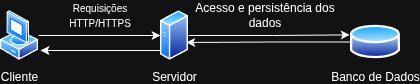
\includegraphics[width=0.5\linewidth]{Imagens/chap04/diagrama_cliente_servidor.png}
    \caption{Representação da arquitetura modular do sistema: cliente, servidor e banco de dados}
    \label{fig:arquitetura_cliente_servidor}
\end{figure}

\section{Arquitetura Limpa}
A arquitetura limpa é uma abordagem de organização de software que busca separar as responsabilidades do sistema em camadas, reduzindo o acoplamento entre regras de negócio, tecnologias externas e mecanismos de entrada e saída. Dessa forma, a lógica central da aplicação não fica dependente diretamente de frameworks, banco de dados, interfaces gráficas ou protocolos de comunicação. Essa separação favorece a manutenção, os testes e a evolução do sistema, pois alterações em uma tecnologia específica não afetam diretamente as regras principais do domínio. A arquitetura é estruturada em camadas bem definidas, cada uma com responsabilidades específicas e com dependências direcionadas para o núcleo do sistema, garantindo que as regras de negócio permaneçam independentes de detalhes externos \cite{sommerville2016,swebok2024}.

Seguindo esses princípios, a camada domain representa o núcleo da aplicação, sendo responsável por conter as entidades, regras de negócio e abstrações fundamentais do sistema, sem depender de tecnologias externas. A camada application atua como intermediária entre o domínio e as demais camadas, coordenando os casos de uso e definindo contratos para a execução das operações do sistema. A camada infrastructure é responsável por implementar detalhes técnicos, como acesso a banco de dados, integração com serviços externos e configurações necessárias para o funcionamento da aplicação. Por último, a camada web corresponde à interface de comunicação com o usuário ou outros sistemas, sendo responsável por receber requisições, encaminhá-las para as camadas internas e retornar as respostas apropriadas.

\section{Camadas da Arquitetura do Sistema}

\subsection{Backend}

O backend corresponde à camada responsável pelo processamento das regras de negócio, pela validação dos dados recebidos, pelo controle de acesso e pela comunicação com os mecanismos de armazenamento e processamento de informações. Essa camada concentra a lógica central do sistema, garantindo que as operações sejam executadas de maneira consistente, segura e de acordo com os requisitos funcionais e não funcionais estabelecidos. Entre suas principais responsabilidades, destacam-se o tratamento e a persistência dos dados, a aplicação de restrições e validações, o gerenciamento de autenticação e autorização, o controle das transações, o tratamento de exceções e a disponibilização de serviços para outras camadas da arquitetura. Além disso, o backend contribui para atributos como integridade, confiabilidade, escalabilidade, segurança e manutenibilidade, constituindo um elemento fundamental para o funcionamento adequado de sistemas computacionais \cite{sommerville2016,swebok2024,iso25010_2023}.

\subsection{Banco de Dados}

O banco de dados é o componente responsável pelo armazenamento persistente, pela organização e pela recuperação das informações utilizadas por um sistema. Trata-se de um elemento fundamental em aplicações computacionais, pois fornece a base necessária para o registro, a manutenção e o acesso estruturado aos dados. Além de armazenar informações de forma duradoura, o banco de dados também contribui para a integridade, a consistência, a segurança e a disponibilidade dos dados, permitindo que eles sejam consultados, atualizados e relacionados de maneira eficiente. Dessa forma, esse componente sustenta o funcionamento das demais camadas do sistema, servindo de apoio para o processamento realizado pela lógica da aplicação e para a disponibilização das informações aos usuários \cite{sommerville2016,swebok2024}.


\subsection{Frontend}

O frontend corresponde à camada de apresentação do sistema, ou seja, à interface gráfica por meio da qual os usuários interagem com a aplicação. É nessa camada que se encontram os elementos visuais e interativos que possibilitam o uso do sistema, como telas, formulários, menus, listagens, botões e mecanismos de navegação. Sua principal função é apresentar informações e funcionalidades de forma compreensível, organizada e acessível, permitindo que a interação do usuário com o sistema ocorra de maneira eficiente e adequada ao seu contexto de uso. Além disso, o frontend contribui para a usabilidade, a clareza na comunicação das informações e a responsividade da interface gráfica, entendida como a capacidade de adaptar a apresentação a diferentes tamanhos de tela e dispositivos. Essa camada também medeia as ações do usuário e os serviços disponibilizados pelas demais partes da arquitetura \cite{sommerville2016,swebok2024,iso25010_2023}.

% 

\section{Ferramentas de Apoio ao Desenvolvimento}

\subsection{Controle de Versão}

O controle de versão é uma prática fundamental no desenvolvimento de software, pois permite registrar, organizar e acompanhar as alterações realizadas no código-fonte ao longo do tempo. Por meio desse processo, torna-se possível recuperar versões anteriores, comparar modificações, identificar a autoria das mudanças e manter um histórico estruturado da evolução do sistema. Além disso, o controle de versão desempenha papel essencial no trabalho colaborativo, uma vez que possibilita que diferentes desenvolvedores atuem simultaneamente sobre o mesmo projeto de forma coordenada, reduzindo conflitos e favorecendo a integração contínua das contribuições. Dessa maneira, essa prática contribui para a rastreabilidade, a segurança, a manutenção e a evolução consistente do software \cite{chacon2014}.


\subsection{Integração Contínua (CI) e Entrega Contínua (CD)}

A integração contínua (Continuous Integration -- CI) e a entrega contínua (Continuous Delivery -- CD) são práticas distintas e complementares de automação do ciclo de desenvolvimento. A CI está associada à incorporação recorrente de mudanças em um repositório compartilhado, normalmente acompanhada da execução automática de testes e validações. A CD se relaciona à preparação do software para que novas versões possam ser disponibilizadas de maneira rápida, consistente e controlada. Em conjunto, essas práticas reduzem procedimentos manuais, favorecem a detecção antecipada de falhas e aumentam a previsibilidade das liberações \cite{gitlabcicd2026}.

\subsection{Conteinerização e Deploy }

A conteinerização consiste em empacotar aplicações, bibliotecas, arquivos de configuração e demais dependências em unidades padronizadas de execução, denominadas contêineres. Essa abordagem permite que o software seja executado de forma mais consistente em diferentes ambientes computacionais, reduzindo incompatibilidades entre desenvolvimento, teste e produção. Ao isolar a aplicação e os elementos necessários ao seu funcionamento, a conteinerização favorece a portabilidade, a padronização e a reprodutibilidade, além de contribuir para a escalabilidade, a eficiência na implantação e a simplificação do gerenciamento dos ambientes. Dessa forma, constitui uma prática amplamente adotada para tornar a distribuição e a execução de sistemas mais previsíveis, controladas e independentes das particularidades da infraestrutura subjacente \cite{docker2026}.
